%%% The main file. It contains definitions of basic parameters and includes all other parts.

%% Settings for single-side (simplex) printing
% Margins: left 40mm, right 25mm, top and bottom 25mm
% (but beware, LaTeX adds 1in implicitly)
\documentclass[12pt,a4paper]{report}
\setlength\textwidth{145mm}
\setlength\textheight{247mm}
\setlength\oddsidemargin{15mm}
\setlength\evensidemargin{15mm}
\setlength\topmargin{0mm}
\setlength\headsep{0mm}
\setlength\headheight{0mm}
% \openright makes the following text appear on a right-hand page
\let\openright=\clearpage

%% Settings for two-sided (duplex) printing
% \documentclass[12pt,a4paper,twoside,openright]{report}
% \setlength\textwidth{145mm}
% \setlength\textheight{247mm}
% \setlength\oddsidemargin{14.2mm}
% \setlength\evensidemargin{0mm}
% \setlength\topmargin{0mm}
% \setlength\headsep{0mm}
% \setlength\headheight{0mm}
% \let\openright=\cleardoublepage

%% Generate PDF/A-2u
\usepackage[a-2u]{pdfx}

%% Character encoding: usually latin2, cp1250 or utf8:
\usepackage[utf8]{inputenc}

%% Prefer Latin Modern fonts
\usepackage{lmodern}

%% Further useful packages (included in most LaTeX distributions)
\usepackage{amsmath}        % extensions for typesetting of math
\usepackage{amsfonts}       % math fonts
\usepackage{amsthm}         % theorems, definitions, etc.
\usepackage{bbding}         % various symbols (squares, asterisks, scissors, ...)
\usepackage{bm}             % boldface symbols (\bm)
\usepackage{graphicx}       % embedding of pictures
\usepackage{fancyvrb}       % improved verbatim environment
\usepackage{natbib}         % citation style AUTHOR (YEAR), or AUTHOR [NUMBER]
\usepackage[nottoc]{tocbibind} % makes sure that bibliography and the lists
			    % of figures/tables are included in the table
			    % of contents
\usepackage{dcolumn}        % improved alignment of table columns
\usepackage{booktabs}       % improved horizontal lines in tables
\usepackage{paralist}       % improved enumerate and itemize
\usepackage{xcolor}         % typesetting in color

\usepackage{pdfpages} % MY PACKAGE: inserting other pdf pages
\usepackage{subcaption} % MY PACKAGE: subfigures

%%% Basic information on the thesis

% Thesis title in English (exactly as in the formal assignment)
\def\ThesisTitle{Semi-supervised Learning in Optical Music Recognition}

% Author of the thesis
\def\ThesisAuthor{Jiří Mayer}

% Year when the thesis is submitted
\def\YearSubmitted{2022}

% Name of the department or institute, where the work was officially assigned
% (according to the Organizational Structure of MFF UK in English,
% or a full name of a department outside MFF)
\def\Department{Institute of Formal and Applied Linguistics}

% Is it a department (katedra), or an institute (ústav)?
\def\DeptType{Department}

% Thesis supervisor: name, surname and titles
\def\Supervisor{doc. RNDr. Pavel Pecina, Ph.D.}

% Supervisor's department (again according to Organizational structure of MFF)
\def\SupervisorsDepartment{Institute of Formal and Applied Linguistics}

% Study programme and specialization
\def\StudyProgramme{Computer Science - Software and Data Engineering}
\def\StudyBranch{ISDP}

% An optional dedication: you can thank whomever you wish (your supervisor,
% consultant, a person who lent the software, etc.)
\def\Dedication{%
Dedication.
}

% Abstract (recommended length around 80-200 words; this is not a copy of your thesis assignment!)
\def\Abstract{%
Optical music recognition (OMR) is a niche subfield of computer vision, where some labeled datasets exist, but there is an order of magnitude more unlabeled data available. Recent advances in the field happened largely thanks to the adoption of deep learning. However, such neural networks are trained using labeled data only. Semi-supervised learning is a set of techniques that aim to incorporate unlabeled data during training to produce more capable models. We have modified a state-of-the-art object detection architecture and designed a semi-supervised training scheme to utilize unlabeled data. These modifications have successfully allowed us to train the architecture in an unsupervised setting, and our semi-supervised experiments indicate improvements to training stability and reduced overfitting.
}

% 3 to 5 keywords (recommended), each enclosed in curly braces
\def\Keywords{%
{optical music recognition}, {semi-supervised learning}, {deep neural network}
}

%% The hyperref package for clickable links in PDF and also for storing
%% metadata to PDF (including the table of contents).
%% Most settings are pre-set by the pdfx package.
\hypersetup{unicode}
\hypersetup{breaklinks=true}

% Definitions of macros (see description inside)
\include{macros}

% Title page and various mandatory informational pages
\begin{document}
\include{title}

%%% A page with automatically generated table of contents of the master thesis

\tableofcontents

%%% Each chapter is kept in a separate file
\chapter{Introduction}
\label{chap:Introduction}

An~example citation: \cite{Andel07}

\chapter{Related Work}
\label{chap:RelatedWork}

\section{The U-Net architecture}

The article \emph{U-Net: Convolutional Networks for Biomedical Image Segmentation} (\cite{UNet}) introduces a fully-convolutional neural network, that is surprisingly good at performing image segmentation. The article uses this architecture for semantic segmentation and instance segmentation of various biomedical images.

\begin{figure}[ht]
    \centering
    \includegraphics[width=145mm]{../img/u-net-architecture.png}
    \caption{The U-Net architecture with a contracting path and an expansive path. The image is taken from \cite{UNet}.}
    \label{fig:UNetArchitecture}
\end{figure}

The authors describe the left part of the network as the contracting path. It follows the typical structure of a convolutional network. The right part is called the expansive path. It is built as an inverse to the contractive part. The combination of contraction and expansion causes the network to first gather context information around each point of the image and then spread it back out to inform the segmentation process. The two halves are connected using skip-connections, so that the expansive path also has accurate local information available. Since the architecture resembles an autoencoder, we refer to the two halves of the network as an encoder and a decoder. One additional advantage of this architecture is its speed of both inference and training.


\section{Music object detection}

A variation of the U-Net architecture has been first utilized in the context of music recognition in the article \emph{On the Potential of Fully Convolutional Neural Networks for Musical Symbol Detection} (\cite{DorferEtAl}). Authors used it for notehead detection, as a continuation of their previous research into convolutional neural networks for music symbol detection. They managed to outperform other approaches with a much simpler system and faster inference time.

\begin{figure}[ht]
    \centering
    \includegraphics[width=145mm]{../img/muscima-detection-comparison.png}
    \caption{Comparison of the R-CNN and the U-Net architecture for object detection on the MUSCIMA++ dataset. The RetinaNet signle-shot detection is very poor, so the image is omitted to save space. The original image with additional images showing other datasets can be found in (\cite{PachaBaseline}).}
    \label{fig:MuscimaDetectionComparison}
\end{figure}

Both authors then refined the approach in the article \emph{Towards Full-Pipeline Handwritten OMR with Musical Symbol Detection by U-Nets} (\cite{HajicEtAl}). The architecture was extended to perform multi-class segmentation in one pass and domain-specific tricks have been added to increase performance on some symbols. A notation assembly system was designed using decision trees and a complete pipeline with MIDI output was constructed and evaluated.

In the same year, a comparison of object detection architectures for musical symbols was published: \emph{A Baseline for General Music Object Detection with Deep Learning} (\cite{PachaBaseline}). The authors trained three object detection architectures, namely Faster R-CNN, RetinaNet, and U-Net. Their evaluation was performed using three datasets with object detection ground truth, and varied appearance and content. These were the Capitan dataset (mensural notation), the DeepScores dataset (digitally printed modern notation), and the MUSCIMA++ dataset (handwritten modern notation). The article establishes baseline results in different areas of music recognition, but most importantly, identifies the U-Net architecture as the best known architecture for object detection.


\section{Generative semi-supervised learning}

TODO: All the unsupervised, semi-supervised, clustering and disentagnling features of adversarial autoencoders (\cite{AdversarialAutoencoders}). Pioneered by smisup VAE (\cite{KingmaSslVae}).

% adversarial autoencoders
% which has been pioneered by M1+M2 VAE

\chapter{Optical Music Recognition}
\label{chap:OMR}

This chapter contains an introduction to optical music recognition (OMR). Most of its content is based on the article \emph{Understanding Optical Music Recognition} (\cite{UnderstandingOmr}).

The article defines OMR as \emph{a field of research that investigates how to computationally read music notation in documents}. This definition attempts to clearly define the term. OMR is a field of research, therefore it encapsualtes the investigation of many problems -- it is not a single task. OMR attempts to computationally read music; it applies existing understanding of various music notations and does not study these notations as such. Recognized documents may be of many types (scanned, digitally-engraved, printed, handwritten, captured from a stylus) and be represented in different music notations (common western, mensural, tablature). This thesis focuses on reading entire pages of handwritten music, expressed in the common western music notation.

The recognition process on its own is also not very useful. It serves as one phase of solving some larger problem, like metadata extraction, archive searching, audio replay, editing or conversion to some other music data format. Each one of these applications has a different set of priorities regarding the recognition. If the goal is to seach by melody, we do not need to recognize rhythm; if the goal is audio replay, we do not need to read lyrics.

It should be noted, that there is a difference between recovering musical semantics and recovering music notation. This stems from the specifics of how music notation encodes musical ideas. Musical symbols on a staff compete for space and this influences their relative position. In music notation, there is also a lot of freedom in how a musical idea is expressed. Some rhytmic phrases may be expressed using either duration dots or using ties and the choice may depend on the writer's preference or on the rhytmic context. Recovering music notation is the easier task of reading individual notation symbols and their relationships. Recovering musical semantics requires an additional step of interpreting the parsed musical notation.

\begin{figure}[ht]
    \centering
    \includegraphics[width=145mm]{../img/music-monophonic.png}
    \includegraphics[width=145mm]{../img/music-pianoform.png}
    \caption{Comparison of monophonic music (top) to a pianoform (bottom). Monophonic music contains only a single voice and can be represented sequentially. Pianoform contains multiple voices spread out over two staves, making it behave more like a graph. The image is taken from (\cite{UnderstandingOmr}).}
    \label{fig:MusicComplexity}
\end{figure}

It is only natural to ask about the relationship of OMR and text recognition. Both fields attempt to read documents containing sequential data and there are many other similarities. However, music recognition is much more difficult for multiple reasons. Music notation is contextual, meaning that interpretation of some symbols depends on other symbols around it. Pitch of a note is one example. We need to know both the key signature (correctly read the clef and accidentals at the beggining of the staff) vertical note position (in relation to staff lines) and possibly an additional accidental in front of the notehead. Size and shape of symbols varies from very small (a dot) to relatively large (beams, slurs, hairpins) to spanning the entire page (tall barlines or braces). Lastly, a single staff of music can contain multiple voices and a pianoform may contain two to three voices on two staves and some notation symbols may be present on both staves simultaneously. Text recognition usually does not need to deal with such a level of complexity.


\section{Approaches to OMR}

Traditional recognition systems relied on the detection of individual symbols and their classification. Stafflines intersect the majority of all symbols, which posed a problem to most object detectors that relied on finding connected components. For this reason, staffline removal was an important preprocessing step.

In recent years, deep learning has been applied to many OMR problems with great success. Especially symbol classification and staffline removal have been considerably improved (\cite{StafflineDetection}, \cite{PachaClassification}). Convolutional neural networks are well capable of learning handwritten symbol classification despite the variance in handwriting styles. In fact, they are able to perform classification without the need for staffline removal -- aggregating multiple phases of a traditional pipeline and greatly simplifying the task.

The pipeline for music recognition has been refined over the years (\cite{BainbridgeBell}, \cite{RebeloSota}) and has currently reached a form with four distinct stages:

\begin{itemize}
    \item \textbf{Preprocessing} Methods that enhance the raw scanned or photographed document for easier processing. These contain perspective compensation, page cropping, contrast enhancement, binarization, noise removal. Basic layout analysis (such as staff detection) also belongs here.
    \item \textbf{Music Object Detection} Finding and classifying all notation symbols.
    \item \textbf{Notation Assembly} Identifying relations between detected symbols and constructing a machine-readable representation (a sequence or a graph).
    \item \textbf{Encoding} Reading and interpreting the recognised notation to fulfil the given task (conversion to another format, audio replay, ...).
\end{itemize}

The introduction of deep learning has allowed an alternative approach to be developed, where all of these stages are performed by a single model. This end-to-end approach has yielded state-of-the-art results in other fields, such as handwritten text recognition (\cite{Scheidl}). It has also been tried for music recognition (\cite{Primus}, \cite{Mayer}), but modelling the complex graph-like structure of music notation is problematic, and so this approach has been limited to monophonic music (which can be represented sequentially).

This thesis focuses on semantic segmentation, which is used as the first step of the object detection stage.


\section{Datasets}
\label{sec:Datasets}

With the shift towards machine learning, several datasets have been created to allow machine learning models to be trained. This thesis relies on three of these datasets:

\begin{itemize}
    \item CVC-MUSCIMA (\cite{CvcMuscima})
    \item MUSCIMA++ (\cite{MuscimaPP})
    \item DeepScores v2 (\cite{DeepScores})
\end{itemize}

These are the only datasets in the OMR field that contain semantic segmentation labels (for Common Western Music Notation). A comprehensive list of other available OMR datasets is maintained by Alexander Pacha on his GitHub page\footnote{\url{https://apacha.github.io/OMR-Datasets/}}.


\subsection{CVC-MUSCIMA}

\begin{figure}[ht]
    \centering
    \includegraphics[width=145mm]{../img/cvc-muscima.png}
    \caption{One page from the CVC-MUSCIMA dataset. The image is taken from the website \url{http://www.cvc.uab.es/cvcmuscima/index_database.html}}
    \label{fig:CvcMuscima}
\end{figure}

This dataset was introduced in the article \emph{CVC-MUSCIMA: A ground truth of handwritten music score images for writer identification and staff removal} (\cite{CvcMuscima}). It contains 1000 pages of handwritten music, created by having 50 writers transcribe 20 unique music pages. It was designed for the tasks of staff removal and writer identification. It is also the only handwritten music dataset, consisting of entire music pages -- all other handwritten datasets contain only individual symbols. This makes it very important for research focusing on symbol detection.

Since the dataset does not contain segmentation labels, we will use it primarily as a source of unlabeled training data.


\subsection{MUSCIMA++}

MUSCIMA++ was created by Jan Hajič jr. and Pavel Pecina as a general-purpouse OMR dataset. It was introduced in the article \emph{In Search of a Dataset for Handwritten Optical Music Recognition: Introducing MUSCIMA++} (\cite{MuscimaPP}). The dataset builds on top of the CVC-MUSCIMA dataset, providing rich annotations for 140 selected pages. The annotation scheme was designed to be sufficiently low-level for tasks such as object detection (bounding boxes, symbol classes, segmentation masks), while also having relationship data in the form of an oriented graph, that lets a user extract semantic information about the music. Dataset authors call this annotation scheme the \emph{Music Notation Graph} (MuNG).

\begin{figure}[ht]
    \centering
    \includegraphics[width=70mm]{../img/muscima-pp.png}
    \caption{Annotations present in the MUSCIMA++ dataset (bounding boxes, segmentation masks and the notation graph). The image is taken from \cite{MuscimaPP}}
    \label{fig:MuscimaPP}
\end{figure}

The dataset was updated in 2019, fixing bugs and modifying class names to be aligned with the SMuFL\footnote{\url{https://www.smufl.org/}} standard. A similar update was also performed on the DeepScores dataset (\cite{DeepScores}), making it easier to use both datasets simultaneously. The latest dataset description and accompanying tools can be found on the GitHub page\footnote{\url{https://github.com/OMR-Research/muscima-pp}} of the OMR Research group\footnote{\url{https://omr-research.net/}}.

We will use this dataset as a source of labeled data for semantic segmentation.


\subsection{DeepScores}

The version 2 of this dataset was introduced in the article \emph{The DeepScoresV2 Dataset and Benchmark for Music Object Detection} (\cite{DeepScores}). The dataset contains entire pages of printed music, with annotations best suited for object detection, semantic segmentation and object classification. It was created from MusicXML documents taken from the MuseScore\footnote{\url{https://musescore.com/sheetmusic}} website and engraved using the LilyPond\footnote{\url{https://lilypond.org/}} tool. The dataset contains 255,386 pages of music, but also provides a dense and diverse subset, having only 1,714 pages. The version 2 also introduced a MUSCIMA++ compatibility mode, making it easier for the two datasets to be used simultaneously.

\begin{figure}[ht]
    \centering
    \includegraphics[width=145mm]{../img/deepscores.png}
    \caption{An example of semantic segmentation labels from the DeepScores v2 dataset. The dataset is very large, but digitally engraved.}
    \label{fig:DeepScoresV2}
\end{figure}

We will use this dataset as a source of labeled data for semantic segmentation.

\chapter{Semi-supervised Learning}
\label{chap:SemisupervisedLearning}

This chapter provides an introduction to and an overview of semi-supervised learning (SSL). The following text draws information predominantly from the article \emph{An Overview of Deep Semi-Supervised Learning} (\cite{SemisupervisedOverview}) and from the book \emph{Semi-supervised learning} (\cite{SslBook}).

In deep learning, the goal typically is to learn some function $f: X \rightarrow Y$ by training a neural network on pairs of data points $(x, y)$. Deep neural networks have large number of trainable parameters, which require adequately large training datasets. Not having enough training data causes the model to overfit and then be unable to generalize to unseen data. Producing training datasets requires a lot of manual labour. Obtaining input data from the domain $X$ is typically easy, the difficult task is assigning correct outputs from $Y$ (called labeling). For this reason, many niche domain problems (e.g. handwritten music recognition or cuneiform recognition) lack sufficiently large labeled datasets for training deep learning models (\cite{MuscimaPP}, \cite{Cuneiforms}). These domains, however, have a relative abundance of unlabeled data.

Semi-supervised learning is a set of methods that aim to utilize this unlabeled data in addition to the available labeled data. The goal of these methods is to produce models that perform better, than models trained on the labeled data alone. The field of SSL has emerged in 1970s and has since accumulated a number of techniques. This thesis focuses on a subset of these techniques, that are based on generative models. However, this chapter provides a short overview of other available techniques as well.

\begin{figure}[p]
    \centering
    \includegraphics[width=140mm]{../img/mnist-manifold.png}
    \caption{Variational autoencoder learns to project 784-dimensional space of MNIST images down to only 2 dimensional space. We can see clusters of individual classes, forming high-density regions and being separated by low-density regions.}
    \label{fig:MnistManifold}
\end{figure}

\begin{figure}[p]
    \centering
    \includegraphics[width=50mm]{../img/decision-boundary.png}
    \caption{Visualization of a classification task, with the decision boundary visible in between the two classes (the while region).}
    \label{fig:DecisionBoundary}
\end{figure}

\qquad

The following text uses a couple of terms, that should be explained first. We will do that on an example:

The figure \ref{fig:MnistManifold} shows the latent space of a variational autoencoder trained on the MNIST dataset (\cite{VariationalAutoencoder}, \cite{Mnist}). The dataset contains grayscale images of handwritten digits, 28x28 pixels in size. In machine learning, the \emph{manifold hypothesis} states, that \emph{real-world high-dimensional datasets lie along low-dimensional manifolds inside that high-dimensional space}. The space of all 28x28 images is such a \textbf{high-dimensional space} (784 dimensions). Manifold, mathematically speaking, is a continuous, locally-eucleidian space (e.g. a plane, sphere, 3D space, Möbius strip). The latent space of the autoencoder is a 2D plane (as seen in the figure \ref{fig:MnistManifold}) and it is the stated \textbf{low-dimensional manifold} containing all the data. The data lies on this manifold, the model has only learned, how this 2D manifold is embeded inside the 784-dimensional space. (Note that it is not the only manifold the data lies on, this is just the one the neural network discovered during training.)

Items of the dataset are not evenly scattered throughout the high-dimensional space. They are coalesced into groups called \textbf{clusters}. Points within these clsuters are located relatively close to each other and usually share the same class. This is an equivalent statement to saying that all digits 7 look alike. These clusters are clearly visible in the latent space (fig. \ref{fig:MnistManifold}), where they form very distinct blobs. The space, where clusters sit, is refered to as \textbf{high-density regions} -- many items from the dataset are located here. Conversely, the space between clusters, where almost no data points are present, is refered to as \textbf{low-density regions}.

A classification task learns a function that assigns a label to each point of the input space. This label is discrete. We can color the input space according to the assigned label and that would produce regions, where all points have the same label. The place where these regions meet is called the \textbf{decision boundary}. A decition boundary can be seen in figure \ref{fig:DecisionBoundary}. In a well-trained classifier for a well-defined classification problem, this decision boundary should lie in the described low-density regions.


\section{Assumptions}
\label{sec:SslAssumptions}

Before we start using semi-supervised methods, we should first understand assumptions that underpin them. These assumptions are mostly intuitive and are satisfied in almost all real-world problems, however stating them explicitly yields better understanding of these methods.

\begin{itemize}
    \item \textbf{The Smoothness Assumption.} \emph{If two points $x_1$, $x_2$ reside in a high-density region and are close together, then their corresponding outputs $y_1$, $y_2$ should also be close together.} For example, if we have a picture of digit 7, then small variations in its shape and color should still be interpreted as digit 7. The opposite statement also holds; if the two input points are separated by a low-density region, the outputs must be distant from each other. This assumption is primarily helpful in a classification task, not so much in a regression task.
    \item  \textbf{The Cluster Assumption.} \emph{If points are in the same cluster, they are likely to be of the same class.} This assumption connects the classification task to the smoothness assumption. It indirectly states, that the decision boundary is located in low-density regions, because otherwise it would cut a cluster in half, causing close points to fall to different classes (which is a violation of the assumption). This assumption can be used as a motivation for methods that push the decision boundary away from data points, into the low-density regions.
    \item \textbf{The Manifold Assumption.} \emph{The (high-dimensional) data lie (roughly) on a low-dimensional manifold.} The problem with high-dimensional data is that as the number of dimensions increases, the volume of the space grows exponentially. This means that most of the space is not covered by any data points in our dataset and that makes it difficult to learn to classify. This assumption states, that our data points actually lie on a small subspace (manifold) of the entire space and that a projection can be learned, that maps this manifold onto a low-dimensional space. Learning the classification task for this low-dimensional space should be much easier.
\end{itemize}


\section{Methods}
\label{sec:SslMethods}

The following section lists major SSL methods. These methods are often directly based on previously stated assumptions and are not mutually exclusive, in fact most of them can be used simultanously as so-called holistic methods. These are, however, not covered in this chapter.


\subsection{Consistency Regularization}

The core idea of this method is that a small neighborhood of each datapoint should have the same label as that datapoint. This idea follows directly from the cluster assumption. In this method we train the model to minimze distance between a known datapoint $x$ and a perturbed datapoint $\hat{x}$. This training is performed in addition to the usual supervised training. This method does not rely on the corresponding label $y$, instead it trains to minimize the distance between $f(x)$ and $f(\hat{x})$. This lets us utilize all unlabeled data points as well.

The method can be seen as an extension of supervised learning. In supervised learning, we train on individual points and learn the overall shape from them. Here, we train on small neighbourhoods, which makes sure the decision boundary will not come close to any individual datapoint. Further utilization of unlabeled data points in the proximity of labeled data points should force the decision boundary even further away, into low-density regions.


\subsection{Proxy-label Methods}

This is a set of methods, that train a supervised model on the labeled data and then use it in some way to label some of the unlabeled data. These methods are also called \emph{bootstrapping}. To distinguish these later-added labels, they are called \emph{pseudo-labels}.

One of these methods is \emph{self-training}. In self-training, labeled data is used to train a supervised classification model. This model is then used to classify all unlabeled data points and since its output is a softmax layer, we can not only pick the most likely class, but also measure the confidence in that class. We define a threshold $\tau$ and only assign pseudo-labels to data points above this threshold. This process can be repeated, until a stopping condition is met (e.g. there are no more unlabeled points with confidence above $\tau$). The main problem of this method is the inability to correct mistakes made during the labeling step.

\emph{Pseudo-labeling} is a similar method, where the unlabeled data points are also assigned pseudo-labels. In this case, these pseudo-labels are treated as trainable parameters, similar to model parameters, and are optimized together with the model during training. The difficult part is designing a good loss function for pseudo-labels, because applying this method naively causes the pseudo-labels to overfit, due to so-called confirmation bias.


\subsection{Graph-based Methods}

These methods frame the problem in the language of graphs. Data points are represented as vertices of a graph and weighted edges are present between pairs of vertices, where the weight corresponds to some similarity between the two points. The labeling task can be viewed as a propagation of information along edges of the graph.

This propagation resembles proxy-label methods, however due to the graph framing, we can consider entities, such as vertex neighbourhood and its impact on the examined node, or we can leverage algebraic structures, like the adjacency matrix.

A different set of graph methods aims to learn data point embeddings, which preserve the structure of the input graph. The goal is to represent each vertex (data point) as a low-dimensional vector, where a simple similarity function (e.g. inner product) would yield similar closeness values as a more complex similarity function in the input space. This again resembles deep learning techniques, such as autoencoding (see figure \ref{fig:MnistManifold}), however here, methods derived from graph theory are used to produce these embeddings (e.g. Laplacian Eigenmaps or Locally Linear Embeddings).


\subsection{Entropy Minimization}

Consistency regularization methods attempt to push the decision boundary away from clusters and into the low-density regions by stabilizing the model output in a neighborhood around each data point. Entropy minimization is a different technique that attempts to do the same thing. In entropy minimization, we penalize the model for being unsure about its predictions. Low-confidence predictions are predictions with more than one class having non-zero probability. Such probability distributions have higher entropy than one-hot distributions. By adding a loss term that minimizes entropy of predictions during training, we can make areas around datapoints more stable. This method can not, however, be used alone for high-capacity models (deep neural networks), as it causes the training to overfit. Instead, it may be used as a supplementing technique to another SSL technique.


\section{Generative Methods}
\label{sec:GenerativeSslMethods}

generative model learns p(x), we then use it to learn p(y|x)
supervised -> add unlabeled
unspuervised -> add labels

\subsection{Variational Autoencoders}

variational autoencoder - kingma et al, M1 M2

\subsection{Adversarial Autoencoders}

adversarial autoencoder

\subsection{Generative Adversarial Networks}

TODO


\section{Related Methods}
\label{sec:RelatedSslMethods}

transfer learning, domain adaptation
    multitask learning

\chapter{Methodology}
\label{chap:Methodology}

This chapter describes the motivation and process behind performed experiments. It starts by describing our modified U-Net architecture and a challenges related to its training. The two following sections describe the preparation of the training data. Last section is a brief overview of object recognition metrics and it describes our motivation for using pixelwise F1 score as the evaluation metric.


\section{Architecture}
\label{sec:Architecture}

In the \emph{generative model} approach to semi-supervised learning, one usually starts with a model that can be trained in the unsupervised manner (either an autoencoder or a generative adversarial network; \cite{AutoencodersOverview}, \cite{GAN}) and then extends it to also perform the supervised task. For example, when starting with an autoencoder, one can use the encoder part as a dimensionality reduction mechanism and then build a supervised classification network that classifies the learned embeddings (\cite{KingmaSslVae}).

In our context of music recognition, we are highly motivated to build on top of the U-Net architecture (\cite{UNet}) (figure \ref{fig:ArchitectureCombined}). It has first been used for biomedical image segmentation, however its superiority for object detection in music recognition has been clearly demonstrated by \cite{PachaBaseline}.

The architecture can be viewed as a fully convolutional autoencoder with residual (skip) connections added between the encoder and decoder on every resolution level. The U-Net encoder is a typical fully-convolutional encoder that gradually reduces image dimensions, while increasing the channel count. Such an architecture is able to learn abstract representations of symbols present in the input image. The decoder then tries to go from these abstract representations back to specific ones, while at the same time modifying the reconstruction to fit the learned segmentation task. The core idea behind this architecture is that the decoder can utilize skip connections during upsampling, thereby producing a pixel-perfect segmentation.

\begin{figure}[ht]
    \centering
    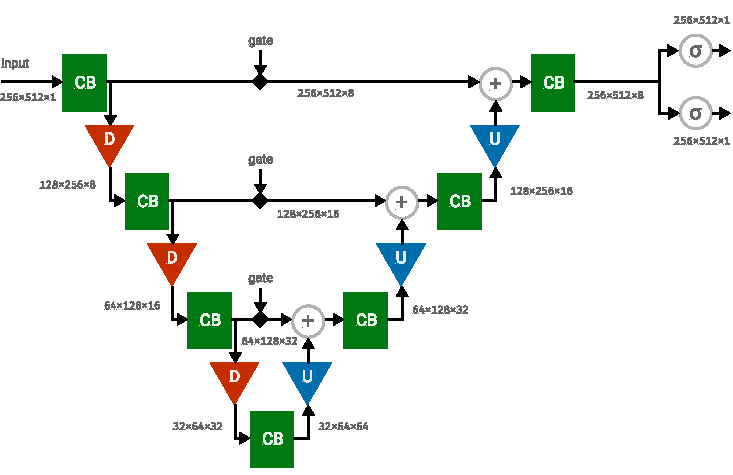
\includegraphics[width=140mm]{../img/architecture-complete.pdf}
    \caption{Block diagram, depicting the used architecture. It has 4 levels, with gated skip connections on each level. The network is forked after the second to last layer to provide separate segmentation and reconstruction outputs. Detailed explanation of each block is provided in figure \ref{fig:ArchitecturePieces}.}
    \label{fig:ArchitectureCombined}
\end{figure}

We choose to share the entire U-Net model for both the supervised and unsupervised tasks. The two tasks are differentiated only at the very last layer. The original U-Net architecture ends with a 1x1 convolution layer with sigmoid activation. It can be viewed as a pixelwise softmax for two output classes (like in a typical classification architecture). We decided to fork the architecture here, having one sigmoid convolution for the supervised segmentation task and one for the unsupervised reconstruction task.

The supervised task can be trained in almost the same way as the the original U-Net archtiecture:

\begin{itemize}
    \item A batch $(x, y)$ of input images and expected segmentation masks is taken from the dataset.
    \item Input images $x$ are fed through the model, producing a prediction for the segmentation mask $\hat{y}$ and for the reconstructed image $\hat{x}$.
    \item A loss function is used, computing the distance between $y$ and $\hat{y}$ and generating gradients for the network.
    \item Reconstruction output $\hat{x}$ is ignored and no gradients for the branch are computed.
    \item An optimizer uses computed gradients to update model parameters.
\end{itemize}

The unsupervised task can be trained in the same way, using the other output branch of the model. The model would receive an image on the input and would be trained to produce an identical image on the reconstruction output. This setup requires no labels, only the music images.

The unsupervised training, as described so far, would work for a typical autoencoder, but since the U-Net architecture contains skip connections, the model could learn an identity function without using any of the abstraction-learning layers. The goal of unsupervised learning is learning these abstract features, so this straightforawrd training scheme is infeasible in our context.

We propose two ways of overcoming this challenge:

\begin{itemize}
    \item gated skip connections
    \item denoising
\end{itemize}

One option is to disable skip connections during reconstruction training and keep them enabled during segmentation training. This should force the model to learn abstract features during reconstruction, while also being able to utilize skip connections during segmentation.

This gated scheme performs better than a plain autoencoder without any skip connections, but the experiment in section \ref{sec:SkipConnections} suggests that having skip connections permanently enabled works better still. Despite this, we choose to use gated skip connections for reasons explained in that section. We combine this gating with the second technique of adding noise.

The denoising option refers to the process of adding noise to the input image, when training the reconstruction task. The model learns to not only reconstruct the input image, but also to remove the added noise. We took inspiration from denoising autoencoders (\cite{StackedDenoisingAutoencoders}). The difficult part is designing the noise function such that it would cause the model to learn abstract representations (see section \ref{sec:NoiseGeneration}).

We consider the described scheme for unsupervised U-Net training to be the main contribution of this thesis. The proposed experiments try to assess the viability of the scheme in the context of semi-supervised learning.

Both the segmentation and reconstruction tasks are trained jointly on composite batches and a single composite loss function. A single optimizer step is used to update model parameters for both tasks somultaneously. The specifics of combining supervised and unsupervised training are described later in section \ref{sec:Training}.

The last sigmoid layers output images with only one channel. For the reconstruction output, this data is interpreted as a grayscale image. For the segmentation output, it represents the probability the model assigns to each pixel of being in the target class. This means that the model can learn to segment only one symbol class.

\cite{HajicEtAl} have explored the option of having multiple segmentation output channels. The hypothesis is that having the model learn multiple classes would improve its accuracy, since some internal representations can be shared. An added advantage is the reduced inference time as multiple segmentation masks can be infered in a single pass. Such a training however introduces problems related to unbalanced class distribution in the training data. Even if these can be overcome, their results suggest minimal accuracy benefits and a risk of decreasing accuracy in some cases.

Despite the fact that our experiments source code lets us easily train multiple classes, we choose not to explore this path as we are interested in the semi-supervised effects only.

\begin{figure}[p]
    \centering
    \includegraphics[width=140mm]{../img/architecture-pieces.pdf}
    \caption{A recursive block schema of the used architecture. When training and infering segmentation, the input images are cropped directly from the given dataset. When training reconstruction, the input images are overlayed with large, tiled noise that zeroes-out some pixels.}
    \label{fig:ArchitecturePieces}
\end{figure}

The figure \ref{fig:ArchitecturePieces} contains a recursive block diagram of our extended U-Net architecture. The model takes a single image as the input and produces both the segmentation mask and the reconstructed image. When training segmentation, the reconstructed image is ignored and when training reconstruction, the input image is covered in noise and the output segmentation is ignored.

Each level of the network begins and ends with a convolutional block (CB). It consists of two identical 3x3 convolutional layers with an optional dropout layer in between them. Both convolutional blocks on the same level output the same number of feature channels. The number of feature channels is dictated by a hyperparameter we call \emph{inner features}. If the network has 4 inner features, the zero-th level convolutions output 4 feature channels. Each successive level then has twice as many feature channels as the one above it (e.g. 4, 8, 16, 32). The figure \ref{fig:ArchitectureCombined} contains image dimensions and channel counts for each edge in the network. The image dimensions are taken with respect to an input image tile of size 512x256.

The downsampling block is implemented as a 2D max pooling layer (\cite{DeepLearningBook}). The number of feature channels is preserved. If we track the feature count through the encoder, we always first double the number of channels in the convolutional block and then reduce the spatial dimensionality in half in the downsampling block. This way the model can learn to extract higher-level features, before the spatial resolution is lowered. Since the image is two dimensional, halving the resolution shrinks the number of pixels to one quarter. Combined with the doubling of channel count, one encoder level effectively discards half of the image data. This acts as a bottleneck, forcing the network to learn relevant high-level representations.

The upsampling block has to perform two operations:

\begin{itemize}
    \item double the spatial dimensions
    \item halve the channel count
\end{itemize}

The resolution increase is performed by nearest neighbour interpolation (each pixel is copied to form a 2x2 region of the output image). The reduction in channel count is performed by a 1x1 convolutional layer, which can be trained to select or combine specific input channels. The upsampling output image may also be padded by zeros, if the desired output resolution is not even (we need to exactly match the resolution of the skip connection).

The gate on the skip connection is implemented as a multiplication by one or zero. This also causes any back-propagating gradients to be zeroed out, when the gate is closed. We took inspiration for the gating implementation from LSTM and GRU cells used in recurrent neural networks (\cite{LSTM}, \cite{GRU}).

The output of the upsampling block and the skip connection is merged in an elementwise sum operation. The original U-Net paper uses concatenation (\cite{UNet}), however \cite{DorferEtAl} have shown that using a sum instead speeds up training, while having minimal impact on model accuracy.

In all layers (except for the two output sigmoid layers) the exponential linear unit (ELU) activation function is used. Reasons for this are described in section \ref{sec:ActivationFunction}.


\section{Combining datasets}

We would like to slice and combine described datasets in various ways, depending on the performed experiment. There are two operations we want to perform:

\begin{itemize}
    \item Split an existing dataset into multiple slices (e.g. validation, supervised and unsupervised slices).
    \item Combine two different datasets together.
\end{itemize}

The splitting is needed for an experiment, that gradually increases the amount of unlabeled data and measures the change in model accuracy. This means the splitting logic has to be stable with respect to the size of the unlabeled slice:

\begin{itemize}
    \item We do not want the content of other slices to change, when we change the size of the unlabeled slice.
    \item We want the unlabeled slice to only gain new data, not to be completely resampled.
\end{itemize}

This stability is achieved by giving consideration to the splitting logic (sampling the unlabeled data as the very last slice) and to the shuffling logic (the data is shuffled prior to splitting). All the randomness in the process is controled by a parameter called \emph{dataset seed}, which is distinct from the plain \emph{seed} used for other initialization (model weights and noise generation). Introduction of the \emph{dataset seed} is essential for isolating our experiments from variability introduced by differential dataset sampling.

One additional consideration has to be made when sampling datasets CVC-MUSCIMA and MUSCIMA++. Because their content consists of music transcribed by 50 different wirters, we would like our splits to keep these writers separate. Anotherwords, we do not want a single writer to be present in both the training set and the validation set. We enforce this constraint to better measure the ability of the trained model to generalize. The official test set of MUSCIMA++ built with this approach is called the \emph{writer-independent test set}, therefore we will call this property of our splitting logic \emph{writer-independence}.

\begin{figure}[ht]
    \centering
    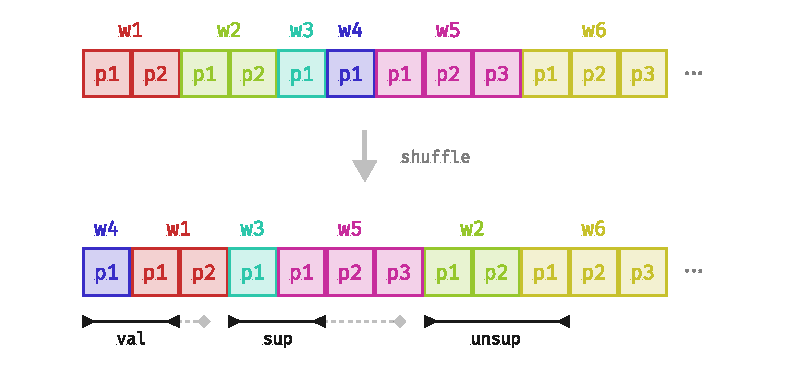
\includegraphics[width=140mm]{../img/dataset-splitting.pdf}
    \caption{Visualization of how a dataset is split in the writer-independent fashion, if we request 2 validation, 2 supervised and 3 unsupervised pages.}
    \label{fig:DatasetSplitting}
\end{figure}

When combining datsets, we run into the problem of image resolution. Since our proposed architecture learns visual features in scale-dependant way, we need to bring all datasets to the same resolution. Datasets CVC-MUSCIMA and MUSCIMA++ have the same source images, so the problem is not present here, however the dataset DeepScores is sampled at a lower resolution. In paper printing, a unit of DPI (dots per inch) is used. We cannot, however, use this unit, since it would assume the music from both datasets has the same size when printed on a paper. A more general approach would be to define a unit, that could be derived from the raster image itself, without any knowledge of the scanning/printing DPI. The open format MusicXML\footnote{\url{https://www.musicxml.com/}} uses a spatial unit defined as \emph{one tenth of interline space} (the distance between two adjacent stafflines). We took inspiration form this and defined a unit we call DPSS (dots per staff space). DPSS of a raster music document is the number of pixels between two neighbouring stafflines. We measured the DPSS of CVC-MUSCIMA to be \verb`28.75 px` and of DeepScores to be \verb`16.0 px`.

\begin{figure}[ht]
    \centering
    \includegraphics[width=140mm]{../img/dpss-definition.pdf}
    \caption{The spatial unit \emph{interline space}, size of which in pixels we call DPSS (dots per staff space).}
    \label{fig:DpssDefinition}
\end{figure}

When matching the resolution of both datasets, we need to perform image resizing and we need to choose the target size and the interpolation method. We ended up upscaling the DeepScores dataset to match the resolution of the CVC-MUSCIMA dataset with the bilinear interpolation method.

In the beginning we tried downscaling CVC-MUSCIMA with area interpolation method. We chose the area method because it does not produce aliasing artifacts (it works by averaging pixel values over an area). It, however, introduced problems with thin lines (such as stafflines and stems) that faded below 50\% intensity on most pixels. That caused the pixelwise F1 score we use to evaluate the experiments to become very noisy and difficult to interpret.


\section{Noise Generation}
\label{sec:NoiseGeneration}

Typical denoising autoencoders are used either for removing noise from existing images (say, an overlayed text, sensor noise, or aliasing artifacts) or for learning abstract features (\cite{StackedDenoisingAutoencoders}). If noise is sufficiently fine, as to not obstruct the high-level structure of the image, the autoencoder can learn this high-level structure in an unsupervised way. This setup can be used for feature extraction, similar to how variational autoencoders are used (\cite{VariationalAutoencoder}).

\begin{figure}[ht]
    \centering
    \includegraphics[width=140mm]{../../figures/06-noise/noise-comparison.pdf}
    \caption{Comparison of various noise sizes. Small nosie is easy for the model to remove and large noise leaves too many possibilites of reconstruction.}
    \label{fig:NoiseComparison}
\end{figure}

Our goal is to leverage this training scheme to force our U-Net model to learn high-level representations. We chose to use noise in the form of dropping out parts of the input image -- setting the image pixels to zero. The parameter that specifies the percentage of zeroed-out image area is called \emph{noise dropout}.

We could decide for each pixel independently, whether it should be dropped, but that would produce a very fine noise. We belive that such a noise would not force the model to learn large symbols, as they are unnecessary for removing the noise. Therefore we chose to increase the resolution of the noise to form a square grid, where one square covers approximately two staff spaces. At this size, dropped regions are large enough, so that simple operations like dilation will not reconstruct them. These regions are also small enough that the number of plausible reconstructions within the dropped space is reasonably limited. An extreme situation would be dropping the entire input image, but there the space of possible reconstructions would be so large, that it would be impossible for the model to guess the correct one (even among the space of plausible reconstructions).

We got the idea of dropping image squares after reading the article by \cite{Cuneiforms}. Authors of the article present a method for reconstructing parts of an input image using a generative adversarial network. Their goal is to create synthetic training data for the task of cuneiform sign recognition.


\section{Evaluation Metrics}
\label{sec:EvaluationMetrics}

Semantic segmentation is closely related to object detection and recognition. It is often performed as the first step from which object bounding boxes are computed. The segmentation output is first binarized by applying a threshold. Adjacent positive pixels are merged to form connected components, where each can then be enclosed in a bounding box. The described process is very basic and there are ways to improve it. A sligtly more advanced process in the context of notehead recognition is used in the article by \cite{DorferEtAl}.

There are many metrics that evaluate the correctness of predicted bounding boxes, comparing them to ground-truth bounding boxes. A metric called intersection over union (IOU) can be used to calculate the overlap of two bounding boxes. Setting a threshold on IOU and computing it between all pairs of predicted and ground-truth bounding boxes lets us compute the binary classification confusion matrix. From this matrix, additional metrics could be computed, such as precision, recall, and F1 score. By introducing a confidence level for each bounding box, or considering the performance over multiple classes, we get a large number of metrics that can be used to assess various aspects of the recognition. An article by \cite{PadillaMetrics} provides an extensive comparison of all these metrics.

Even though these object detection metrics are more telling about the actual usefulness of the model (we care about detected objects, not pixels), we chose to evaluate our experiments directly at the pixel level. Adding these evaluation metrics adds unecesasry complexity to our experiments and it is not needed for our goal -- measuring the impact of unsupervised data.

We chose to use the pixelwise F1 score at 0.5 thresholding. The F1 score is computed as the harmonic mean of precision and recall, so that it is high, when both precision and recall are high. It is computed from the confusion matrix via the following formula:

$$
    F1 = \frac{2 \cdot TP}{2 \cdot TP + FP + FN}
$$

The confusion matrix values are computed over all pixels of the the entire (validation) dataset.

It is important to note, that the two articles regarding music symbol detection (\cite{HajicEtAl}, \cite{DorferEtAl}) use object detection F1 score, which is not directly comparable to our pixelwise F1 score.

\chapter{Experiments and Results}
\label{chap:ExperimentsAndResults}

TODO: quick chapter overview

\begin{code}
$ python3 main.py unet train --val_pages 123 ...
\end{code}


\section{Architecture}
\label{sec:Architecture}

In the \emph{generative model} approach to semi-supervised learning, one usually starts with a model that can be trained in the unsupervised manner (either an autoencoder or a generative adversarial network [CITE, CITE]) and then extends it to also perform the supervised task. For example, when starting with an autoencoder, one can use the encoder part as a dimensionality reduction mechanism and then build a supervised classification network that classifies the learned embeddings [CITE].

In our context of music recognition, we are highly motivated to build on top of the U-Net architecture [CITE] (figure \ref{fig:ArchitectureCombined}). It has first been used for biomedical image segmentation, however its superiority for object detection in music recognition has clearly been demonstrated by Pacha et al. [CITE].

The architecture can be viewed as a fully convolutional autoencoder with residual (skip) connections added between the encoder and decoder on every resolution level. The U-Net encoder is a typical fully-convolutional encoder that gradually reduces image dimensions, while increasing the channel count. Such an architecture is able to learn abstract representations of symbols present in the input image. The decoder then tries to go from these abstract representations back to specific ones, while at the same time modifying the reconstruction to fit the learned segmentation task. The core idea behind this architecture is that the decoder can utilize skip connections during upsampling, thereby producing a pixel-perfect segmentation.

\begin{figure}[ht]
    \centering
    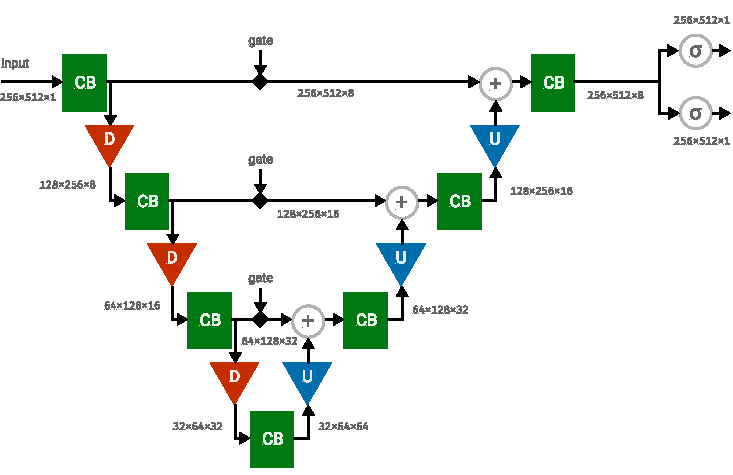
\includegraphics[width=140mm]{../img/architecture-complete.pdf}
    \caption{TODO}
    \label{fig:ArchitectureCombined}
\end{figure}

We choose to share the entire U-Net model for both the supervised and unsupervised tasks. The two tasks are differentiated only at the very last layer. The original U-Net architecture ends with a 1x1 convolution layer with sigmoid activation. It can be viewed as a pixelwise softmax for two output classes of a typical classification model. We decided to fork the architecture here, having one sigmoid convolution for the supervised segmentation task and one for the unsupervised reconstruction task.

The supervised task can be trained in almost the same way as the the original U-Net archtiecture:

\begin{itemize}
    \item A batch $(x, y)$ of input images and expected segmentation masks is taken from the dataset.
    \item Input images $x$ are fed through the model, producing a prediction for the segmentation mask $\hat{y}$ and for the reconstructed image $\hat{x}$.
    \item A loss function is used, computing the distance between $y$ and $\hat{y}$ and generating gradients for the network.
    \item Reconstruction output $\hat{x}$ is ignored and no gradients for the branch are computed.
    \item An optimizer uses computed gradients to update model parameters.
\end{itemize}

The unsupervised task could be trained in the same way, using the other output branch of the model. This would work for a typical autoencoder, but since the U-Net architecture contains skip connections, the model could learn an identity function without using any of the abstraction-learning layers. The goal of unsupervised learning is learning these abstract features, so this training scheme is infeasible in our context.

We propose two ways of overcoming this challenge:

\begin{itemize}
    \item gated skip connections
    \item denoising
\end{itemize}

One option is to disable skip connections during reconstruction training and keep them enabled during segmentation training. This should force the model to learn abstract features during reconstruction, while also being able to utilize skip connections during segmentation. This scheme performs much better than a typical autoencoder without any skip connections, but is still outperformed by the next proposed scheme (see detailed comparison in section \ref{sec:SkipConnections}).

The second option is to add some noise to the input image during reconstruction training. The model would learn to not only reconstruct the input image, but also to remove the added noise. We took inspiration from denoising autoencoders [CITE AUTOENCODERS]. The difficult part is designing the noise function such that it would cause the model to learn abstract representaions (see section \ref{sec:NoiseGeneration}).

We consider the described scheme for unsupervised U-Net training to be the main contribution of this thesis. The proposed experiments try to assess the viability of the scheme in the context of semi-supervised learning.

Both the segmentation and reconstruction tasks are trained jointly on composite batches and a single composite loss function. A single optimizer step is used to update model parameters for both tasks somultaneously. The process is described in detail in section \ref{sec:Training}.

The last sigmoid layers output images with only one channel. For the reconstruction output, this data is interpreted as a grayscale image. For the segmentation output, it represents the probability the model assigns to each pixel of being in the target class. This means that the model can learn to segment only one symbol class.

Hajič et al. [CITE] have explored the option of having multiple segmentation output channels. The hypothesis is that having the model learn multiple classes would improve its accuracy, since some internal representations can be shared. An added advantage is the reduced inference time as multiple segmentation masks can be infered in a single pass. Such a training however introduces problems related to unbalanced class distribution in the training data. Even if these can be overcome, their results suggest minimal accuracy benefits and a risk of decreasing accuracy in some cases.

Despite the fact that our experiment source code lets us easily train multiple classes, we choose not to explore this path as we are interested in the semi-supervised effects only.

\begin{figure}[p]
    \centering
    \includegraphics[width=140mm]{../img/architecture-pieces.pdf}
    \caption{TODO}
    \label{fig:ArchitecturePieces}
\end{figure}

The figure \ref{fig:ArchitecturePieces} contains a recursive block diagram of our extended U-Net architecture. The model takes a single image as the input and produces both the segmentation mask and the reconstructed image. When training segmentation, the reconstructed image is ignored and when training reconstruction, the input image is covered in noise and the output segmentation is ignored.

Each level of the network begins and ends with a convolutional block (CB). It consists of two identical 3x3 convolutional layers with an optional dropout layer in between them. Both convolutional blocks on the same level output the same number of feature channels. The number of feature channels is dictated by a hyperparameter we call \emph{inner features}. If the network has 4 inner features, the zero-th level convolutions output 4 feature channels. Each successive level then has twice as many feature channels as the one above it (e.g. 4, 8, 16, 32). The figure \ref{fig:ArchitectureCombined} contains image dimensions and channel counts for each edge in the network. The image dimensions are taken with respect to an input image tile of size 512x256.

The downsampling block is implemented as a 2D max pooling layer [CITE]. The number of feature channels is preserved. If we track the feature count through the encoder, we always first double the number of channels in the convolutional block and then reduce the spatial dimensionality in half in the downsampling block. This way the model can learn to extract higher-level features, before the spatial resolution is lowered. Since the image is two dimensional, halving the resolution shrinks the number of pixels to one quarter. Combined with the doubling of channel count, one encoder level effectively discards half of the image data. This acts as a bottleneck, forcing the network to learn relevant high-level representations.

The upsampling block has to perform two operations:

\begin{itemize}
    \item double the spatial dimensions
    \item halve the channel count
\end{itemize}

The resolution increase is performed by nearest neighbour interpolation (each pixel is copied to form a 2x2 region of the output image). The reduction in channel count is performed by a 1x1 convolutional layer, that can be trained to select or combine specific input channels. The output may also be padded by zeros, if the desired output resolution is not even (we need to exactly match the resolution of the skip connection).

The gate on the skip connection is implemented as a multiplication by one or zero. This also causes any back-propagating gradients to be zeroed out, when the gate is closed. We took inspiration for the gating implementation from LSTM and GRU cells used in recurrent neural networks [CITE, CIRE].

The output of the upsampling block and the skip connection is merged in an elementwise sum operation. The original U-Net paper uses concatenation [CITE], however Dorfer et al. have shown that using a sum instead speeds up training, while having minimal impact on model accuracy [CITE].

In all layers (except for the two output sigmoid layers) the exponential linear unit (ELU) activation function is used. The reasons for this are described in section \ref{sec:ActivationFunction}.


\section{Datasets}
\label{sec:Datasets}

When performing experiments, we will use these three datasets:

\begin{itemize}
    \item CVC-MUSCIMA [CITE]
    \item MUSCIMA++ [CITE]
    \item DeepScores v2 [CITE]
\end{itemize}

These are the only datasets in the OMR field that contain semantic segmentation labels (for Common Western Music Notation). A comprehensive list of available OMR datasets is maintained by Alexander Pacha on his GitHub page\footnote{\url{https://apacha.github.io/OMR-Datasets/}}.


\subsection{CVC-MUSCIMA}

This dataset was introduced in the article \emph{CVC-MUSCIMA: A ground truth of handwritten music score images for writer identification and staff removal} [CITE]. It contains 1000 pages of handwritten music, created by having 50 writers transcribe 20 unique music pages. It was designed for the tasks of staff removal and writer identification. It is also the only handwritten music dataset, consisting of entire music pages -- all other handwritten datasets contain only individual symbols. This makes it very important for research focusing on symbol detection.

\begin{figure}[ht]
    \centering
    \includegraphics[width=140mm]{../img/cvc-muscima.png}
    \caption{One page from the CVC-MUSCIMA dataset. Image taken from the website \url{http://www.cvc.uab.es/cvcmuscima/index_database.html}}
    \label{fig:CvcMuscima}
\end{figure}

Since the dataset does not contain segmentation labels, we will use it primarily as a source of unlabeled training data.


\subsection{MUSCIMA++}

MUSCIMA++ was created by Jan Hajič jr. and Pavel Pecina as a general-purpouse OMR dataset. It was introduced in the article \emph{In Search of a Dataset for Handwritten Optical Music Recognition: Introducing MUSCIMA++} [CITE]. The dataset builds on top of the CVC-MUSCIMA dataset, providing rich annotations for 140 selected pages. The annotation scheme was designed to be sufficiently low-level for tasks such as object detection (bounding boxes, symbol classes, segmentation masks), while also having relationship data in the form of an oriented graph, that lets a user extract semantic information about the music. Dataset authors call this annotation scheme the \emph{Music Notation Graph} (MuNG).

\begin{figure}[ht]
    \centering
    \includegraphics[width=100mm]{../img/muscima-pp.png}
    \caption{Annotations present in the MUSCIMA++ dataset (bounding boxes, segmentation masks and the notation graph). The image is taken from [CITE]}
    \label{fig:CvcMuscima}
\end{figure}

The dataset was updated in 2019, fixing bugs and modifying class names to be aligned with the SMuFL\footnote{\url{https://www.smufl.org/}} standard. A similar update was also performed on the DeepScores dataset [CITE], making it easier to use both datasets simultaneously. The latest dataset description and accompanying tools can be found on the GitHub page\footnote{\url{https://github.com/OMR-Research/muscima-pp}} of the OMR Research group\footnote{\url{https://omr-research.net/}}.

We will use this dataset as a source of labeled data for semantic segmentation.


\subsection{DeepScores}


\subsection{Data pipeline}

% - MUSCIMA++
% - DeepScores
% - solving resolution problems
% - solving stability (dataset seed) when increasing unsupervised ratio (fixing sup split, growing unsup split)


\section{Noise Generation}
\label{sec:NoiseGeneration}

% - why large noise -> to learn representaions?
% - mention cuneiform article from ICDAR - GAN reconstruction
% - noise generation and parameters


\section{Training}
\label{sec:Training}

% - image tiles / tile size
% - composite batches
% - what input/output combinations we will use
% - training both simultaneously
% - loss function
% - pick the model with the lowest validation loss over a training session


\section{Evaluation Metrics}
\label{sec:EvaluationMetrics}

% - F1 score
% - pixelwise vs. object detection
%     - reference other works and their approach
%     - pixelwise isn't directly telling about object detection performance
% - thresholding due to varying image resolution

% - object detection metrics overview:
%     https://towardsdatascience.com/evaluating-performance-of-an-object-detection-model-137a349c517b


\section{Semi-supervised Improvements}
\label{sec:SemisupervisedImprovements}

The main hypothesis this work is attempting to validate is that adding unlabelled data to the training process helps. We primarily want to improve model accuracy, but as we will see, this is not what our experiments suggest. They do, however, show improvements in other areas, such as training stability and reduced overfitting (section \ref{sec:UtilizingCvcMuscima}).

In the first experiment, we test how various labeled to unlabeled data ratios affect the training process. The experiment uses the MUSCIMA++ dataset [CITE]:

\begin{itemize}
    \item 10 pages act as the labeled set.
    \item 0, 5, 10 and 50 pages act as the unlabeled set.
    \item 10 pages act as the validation set.
    \item All of these pages come from the writer-independent train set of MUSCIMA++ and are chosen in a writer-independent manner (all the splits contain pages by different writers).
\end{itemize}

The learned task is notehead segmentation (both full and empty noteheads). Noteheads are an ideal symbol for this kind of measurement. Firstly, they are very abundant. Each page of the dataset contains many instances of them and they are evenly scattered over the whole page. If we were to instead detect more rare symbols (such as clefs or rests), it could skew the results, making it difficult to separate the effects we want to measure. Handwritten noteheads are also very diverse in style, making them more interesting to learn (compared to, say, stafflines).

All model hyperparameters are set to sensible deafults. The derivation of these values is desribed later in section \ref{sec:UnderstandingHyperparameters}. The model capacity, described by the \emph{inner features} parameter is set to 8, which is useful to know for comparison with the next experiment. The proposed dataset is rather small and so the training is very noisy (figure \ref{fig:ExplorationNoteheadsNoDropout}). To stabilize the trainig we set the dropout parameter to 50\% [CITE DROPOUT].

\begin{figure}[ht]
    \centering
    \includegraphics[width=140mm]{../../figures/01-exploration-noteheads/noteheads.pdf}
    \caption{Training on a small dataset without dropout is noisy, see the orange line at the beginning and the green line at the end.}
    \label{fig:ExplorationNoteheadsNoDropout}
\end{figure}

We expect that as we add more and more unlabeled data, the F1 score should reach higher and higher. Or at least not get worse. This is not what we see in the figure \ref{fig:ExplorationNoteheads}. The fully supervised model outperforms all the others by a clear margin.

Focusing only on the semi-supervised models, it seems that adding more unsupervised data maybe helps here, although the three lines end up on top of each other at the epoch 200. A better idea is to look at the figure \ref{fig:ExplorationNoteheadsEvaluation}. The chart contains evaluation results on the test set of six runs of each configuration. We can clearly see how the performance rises with more unsupervised data. Unfortunately it does not reach above the fully-supervised results. We unfortunately cannot push the amount of unlabeled data much higher, as it would break our training process (see section \ref{sec:BatchSize}) and it would likely also have diminishing returns. The actual numbers are summarized in table \ref{tab:ExplorationNoteheads}.

The reason for the drop in performance is actually caused by the fact, that the supervised model has to only learn one task -- segmentation. Whereas the semi-supervised one has to also learn the unsupervised reconstruction task. This claim is explored in the next section and is supported by the fact that the performance drop disappears when we increase model capacity.

\begin{figure}[p]
    \centering
    \includegraphics[width=140mm]{../../figures/01-exploration-noteheads/noteheads-dropout.pdf}
    \includegraphics[width=140mm]{../../figures/01-exploration-noteheads/noteheads-dropout-smooth.pdf}
    \caption{Lorem ipsum dolor.}
    \label{fig:ExplorationNoteheads}
\end{figure}

\begin{figure}[ht]
    \centering
    \includegraphics[width=140mm]{../../figures/01-exploration-noteheads/noteheads-evaluation.pdf}
    \caption{Lorem ipsum dolor.}
    \label{fig:ExplorationNoteheadsEvaluation}
\end{figure}

\begin{table}[b!]
    \centering
    \begin{tabular}{l@{\hspace{1.5cm}}D{.}{,}{3.2}D{.}{,}{1.2}D{.}{,}{2.3}}
        \toprule
        & \mc{} & \mc{\textbf{Směrod.}} & \mc{} \\
        \pulrad{\textbf{Efekt}} & \mc{\pulrad{\textbf{Odhad}}} & \mc{\textbf{chyba}$^a$} &
        \mc{\pulrad{\textbf{P-hodnota}}} \\
        \midrule
        Abs. člen     & -10.01 & 1.01 & \mc{---} \\
        Pohlaví (muž) & 9.89   & 5.98 & 0.098 \\
        Výška (cm)    & 0.78   & 0.12 & <0.001 \\
        \bottomrule
    \end{tabular}
    \caption{Lorem ipsum dolor.}
    \label{tab:ExplorationNoteheads}
\end{table}

TODO: show visualization images / qualitative comparison between runs?


\section{Utilizing CVC-MUSCIMA}
\label{sec:UtilizingCvcMuscima}

This experiment attempts to address issues of the previous experiment:

\begin{itemize}
    \item fixed model capacity
    \item small dataset
\end{itemize}

In the chapter \ref{chap:CurrentStateOfOMR} we described the two major datasets for handwritten music recognition: CVC-MUSCIMA [CITE] and MUSCIMA++ [CITE]. The dataset MUSCIMA++ is a highly annotated subset of CVC-MUSCIMA. We can view both datasets together as a single semi-supervised dataset, being 12\% labeled and 88\% unlabeled. To the best of our knowledge, nobody has yet tried to utilize both datasets simulatenously for semantic segmentation.

Hajič jr. and Dorfer [CITE 1, 2] have used the U-Net architecture [CITE] for segmentation and they trained it on the MUSCIMA++ dataset. Their results are very impressive. Being able to further build on their work and improving the model by utilizing unlabeled data from CVC-MUSCIMA would be very helpful for the field of OMR. This experiment attempts to do just that.

We take the whole CVC-MUSCIMA dataset, separate writers from the MUSCIMA++ independent test set, separate 20 pages for validation set and remove other pages from these validation writers. The pages that remain are produced by writers not present in both the test set and the validation set. These remaining pages are partially contained in the MUSCIMA++ dataset (99 pages) and all the other pages are used as unlabeled data (551 pages). Therefore we train on 650 out of 1000 pages of the CVC-MUSCIMA dataset.

Since the dataset is now much larger than in the previous experiment (section \ref{sec:SemisupervisedImprovements}), we no longer need the dropout. In fact, the training is even more stable and individual runs are clearly separated.

This experiment attempts to compare fully-supervised and semi-supervised models, regardless of their capacity. We therefore train various model capacities (the \emph{inner features} model parameter) and then compare the best ones for each setting.

Another difference to the previous experiment is that the ratio of labeled to unlabeled data is fixed and given by dataset sizes. The ratio of 99 to 551 pages corresponds best with the ratio 10:50.

\begin{figure}[p]
    \centering
    \includegraphics[width=140mm]{../../figures/01-exploration-noteheads/noteheads-dropout.pdf}
    \includegraphics[width=140mm]{../../figures/01-exploration-noteheads/noteheads-dropout-smooth.pdf}
    \caption{Lorem ipsum dolor. TODO: the two improvements charts}
    \label{fig:CvcImprovements}
\end{figure}

The validation dataset F1 score over the course of training can be seen in figure \ref{fig:CvcImprovements}. In these charts we can see:

\begin{itemize}
    \item Models with 1 and 2 \emph{inner features} are clearly underfitting in the supervised mode (compared to other models). When we add the unlabeled data, their perfomance drops significantly, but the training curve gets much smoother.
    \item Models with 4 and 8 \emph{inner features} worsen much less and also get smoother (especially 4 becomes much more stable).
    \item Model 16 no longer worsens, it is able to learn both tasks.
\end{itemize}

Conclusions can be drawn from these observations:

\begin{itemize}
    \item The reconstruction and segmentation tasks clearly compete for model capacity. The performance drop of adding unlabeled data decreases, as the model capacity increases.
    \item The addition of unlabeled data can be used as a regularization technique. This is evident from the fact that training curves get much smoother as we add unlabeled data. A~regularization effect is also described in the corresponding literature [CITE SSL overview].
    \item All models come close to the 96\% line, but never cross it. While the semi-supervised models get as good as the fully-supervised, they never get better. It seems the reconstruction task is not learning any useful representations. [TODO: expand on this further and show reconstruction visualizations - they learn simple shapes, not abstract objects]
\end{itemize}

% TODO: evaluate best models of SUP and SEMISUP, maybe they differ in test score? Probbably not.


\section{Knowledge Transfer}
\label{sec:KnowledgeTransfer}

TODO: knowledge transfer experiment


\section{Understanding Hyperparameters}
\label{sec:UnderstandingHyperparameters}


\subsection{Batch Size}
\label{sec:BatchSize}

In the deep learning field, it is known that having a small batch size makes the training fast and noisy, whereas a large batch size makes it more stable at the cost of being slower [CITE DL BOOK]. Since our model is fully cconvolutional and we train it on image tiles of fixed size, we can consider the size of these tiles to be a parameter similar to batch size. It also regulates the amount of data used for gradient estimation. If the tiles are large enough, we can get away with batch size of 1 (this is what the original U-Net article does [CITE]).

Using such a small batch size is, however, not possible in our case. Our training process expects batches containing both labeled and unlabeled data. Batch size determines the total number of these two kinds of data items in the single composite batch. The ratio of these two item types within the composite batch is dictated by the ratio within the whole dataset. So if our dataset has, for example, 1:5 labeled to unlabeled data, the batch size has to be at least 6. Otherwise we will start getting batches that contain only unlabeled data. This rule isn't as strict, since the model would probably learn both tasks even if half of all batches were missing labeled data, however if the imbalance becomes too severe, the training fails.

TODO: figure with the failing training (bs=2,ratio=1:10)

An example of such a failing training can be seen in figure TODO???. The model learns to perform reconstruction even for the segmentation task. This is understandable, since the two tasks are differentiated only at the last layer (1x1 sigmoid convolution). If all second-to-last layer activations contain image reconstruction data, then any 1x1 convolution combination of them will do as well.

Since all of our experiments have training data ratios between 1:0 and 1:10, we chose to set the batch size parameter to 10.


\subsection{Dropout}
\label{sec:Dropout}

We introduced dropout [CITE] when training on small datasets (section \ref{sec:SemisupervisedImprovements}). The training was so noisy, that it was difficult to infer any measurable differences between runs. Therefore we used dropout as a mean to stabilize the training. The model performace also sligtly increased in this setting.

When we train on larger datasets, the training is no longer unstable and dropout is not needed (section \ref{sec:UtilizingCvcMuscima}). In fact, it causes the training process to converge much slower (2x or more) and it does not perform any better.

Both the original U-Net article [CITE] and the article by Hajič jr. et al. [CITE] use the U-Net architecture without any dropout. In fact, an article by Thompson et al. [CITE] argues, that using traditional dropout on convolutional layers may not be ideal. This agrees with our findings, that dropout helps only in very specific circumstances.

It may be the case, that using batch normalization instead or dropout (like Hajič jr. et al. [CITE]) has the same effect of regularizing the network. However our goal is not to find the optimal architecture, but to measure the impact of unsupervised data. For that reason we did not explore this option.

From all this we conclude that dropout should be disabled by default.


\subsection{Skip Connections}
\label{sec:SkipConnections}

% chart of the three
% gated works better than none, and solid are better still
% however we are still below fully-supervised, maybe being over would change the order! Disclaim that!


\subsection{Unsupervised Loss Weight}
\label{sec:UnsupervisedLossWeight}

% changes relative learning speed ofthe two tasks, but they get learned nonetheless
% (we say we want segmentation - then reconstruction is also learned, just very slowly)
% + charts show minimal difference when tweaking the value
% when set to 0, fully-supervised mode is entered


\subsection{Noise Parameters}
\label{sec:NoiseParameters}

% noise dropout - for solid connection has little effect -> model learns sup easily
% for gated connection we see an improvement -> model is forced to learn representations
% that actually help it?


\subsection{Activation Function}
\label{sec:ActivationFunction}

We first used ReLU activation function (rectified linear unit) [CITE] in all convolutional layers (except the final sigmoid layer), just like it is used in the original U-Net article [CITE]. However, we occasionally encountered problems with convergence. Replacing the activation function with ELU (exponential linear unit) [CITE] solved these issues. We took inspiration from Hajič jr. et al. [CITE], who also use the ELU activation function. The difference between the two can be seen in figure \ref{fig:ActivationFunctions}.

\begin{figure}[ht]
    \centering
    \includegraphics[width=140mm]{../../figures/03-activation-function/functions.pdf}
    \caption{Visualization of the explored activation functions. ReLU is flat in negative values and therefore has no gradient there. ELU has exponentially decaying gradient and leaky ReLU has a constant gradient. The parameter for the displayed leaky ReLU is 0.1 to make its shape more apparent.}
    \label{fig:ActivationFunctions}
\end{figure}

The convergence problems were happening at the very beginning of training. The model quickly learned to output a completely black image and never recovered from that state. We think it was an instance of the "dying ReLU" problem [CITE]. When the model is first initialized, it outputs a gray-ish image, since model weights are drawn from a uniform distribution centered on zero and the final sigmoid layer turns that into a 0.5 gray. Because the target images have black background, the model first learns to produce mostly black images. Only then does it learn to output white pixels as well (see figure \ref{fig:ActivationTrainingProgression}). With ReLU, the first training phase probably overshoots into the negative range of most synapses and that causes the model to get stuck in that negative range with zero gradient.

\begin{figure}[ht]
    \centering
    \includegraphics[width=140mm]{../../figures/03-activation-function/progression.pdf}
    \caption{The training process starts by learning to output a mostly black image, which probably causes the model to overshoot during the fully-supervised training and get stuck in the "dying ReLU" problem.}
    \label{fig:ActivationTrainingProgression}
\end{figure}

Interestingly enough, this problem happens only when training in the fully-supervised mode. We have never encountered it, when training in the semi-supervised mode. This again suggests that the unlabeled data acts as regularization, damping any extreme gradients, and stabilizing the training.

We also tried using the leaky ReLU function [CITE] with parameter $\alpha = 0.01$, however the problem still remained. Maybe a larger value for $\alpha$ would help, although we already knew that ELU works, so we haven't explored this further.

\begin{figure}[ht]
    \centering
    \includegraphics[width=140mm]{../../figures/03-activation-function/performance.pdf}
    \caption{An experiment from section \ref{sec:UtilizingCvcMuscima} with 8 inner features, trained in fully-supervised mode with various activation functions. All runs show the same performance.}
    \label{fig:ActivationFunctionPerformances}
\end{figure}

We run one of the experiments from section \ref{sec:UtilizingCvcMuscima} with all proposed activation functions to see what impact it has on model performance (figure \ref{fig:ActivationFunctionPerformances}). We can clearly see that they all perform equally well, so we choose ELU as the only activation function that does not suffer from the convergence problem. We thereby validate the work of Dorfer. et al. [CITE] (their article does not provide explanation for the use of ELU, but we belive they must have encountered these exact same problems).

\chapter{Conclusion and Future Work}
\label{chap:ConclusionAndFutureWork}

% - very minor improvements and mostly not in the perfomance, not worth the effor
% - check notes in the thesis-text-structure.md
% - main acomplishment -- ways of training U-Net in an unsupervised manner



% - the improvement is minor and difficult to achieve
% - unsup data does provide regularization
%     - less noisy learning curve
%     - SS coverges, when fully supervised does not
%     - prevents overfitting (expand on what that means)
% From introduction:
% - we found that improvements can be achieved, however they are relatively minor and occur in only very specific circumstances
%     - this is probably because the model learns only low-level features (as seen in denoising visualizations); should it learn higher-level featuers, it could work better (GAN, etc..)
%         - show visualizations, desribe in detail
%         - describe GAN as a learned-loss function


%%% Bibliography
\include{bibliography}

%%% Figures used in the thesis (consider if this is needed)
%\listoffigures

%%% Tables used in the thesis (consider if this is needed)
%%% In mathematical theses, it could be better to move the list of tables to the beginning of the thesis.
%\listoftables

%%% Abbreviations used in the thesis, if any, including their explanation
%%% In mathematical theses, it could be better to move the list of abbreviations to the beginning of the thesis.
%\chapwithtoc{List of Abbreviations}

%%% Attachments to the master thesis, if any. Each attachment must be
%%% referred to at least once from the text of the thesis. Attachments
%%% are numbered.
%%%
%%% The printed version should preferably contain attachments, which can be
%%% read (additional tables and charts, supplementary text, examples of
%%% program output, etc.). The electronic version is more suited for attachments
%%% which will likely be used in an electronic form rather than read (program
%%% source code, data files, interactive charts, etc.). Electronic attachments
%%% should be uploaded to SIS and optionally also included in the thesis on a~CD/DVD.
%%% Allowed file formats are specified in provision of the rector no. 72/2017.
%\appendix
%\chapter{Attachments}

%\section{First Attachment}

\openright
\end{document}
